%%%---------------------------------
%%% CHAPTER TECHNOLOGY OVERWIEV
%%%---------------------------------

\chapter{Technology Overview}
\label{ch:overview}

\section{Cloud Computing Introduction}
In the beginning of computer times, we used dedicated servers to run enterprise applications. One application would run on a single physical machine. These machines could be small servers or large mainframes. When an organization grown and their application required more resources, the server would scale up, which means adding more processors, memory, or storage to the host. This method was not flexible enough, as every change required physical access to the datacentre and buying new hardware. This problem has been solved by virtualization.

Virtualization is a technology that enables running several virtual servers on a single host. Every virtual server would have its own operating system and would act as a physical host. These servers could be dynamically scaled up and down without the need of a physical access to the datacentre. New virtual servers could be provisioned, unused servers could be deleted to make space for scaling, which would reflect the business needs in more flexible way then dedicated servers. This method is also referred to as a traditional virtualization.

\subsection{Difference Between Traditional Virtualisation and Cloud Computing}
In a traditional virtualization, virtual servers are created and managed as part of a single physical host. Virtual machines on every physical host must be managed separately, directly on the host. This approach, again, might not seem flexible enough for large corporations running tens, hundreds, or even thousands of virtual servers on many physical hosts in several datacentres. This is why a technology called cloud computing has emerged.

Cloud computing, in a similar way as traditional virtualization, is a technology that manages running of virtual machines. The main difference is that in cloud computing, a virtual layer of resources, such as computing power, memory, and storage, is created over one or more datacentres. These resources are then used to provision virtual servers. However, it is up to the cloud computing technology to choose on which host the server would run.

This approach is very flexible in terms of creating, deleting, and scaling virtual servers. It also brings new technology, such as software-defined networking, or an object store, both of which will be described later in the thesis.

\subsection{Cloud Applications and Scaling}
The cloud computing flexibility has completely changed the way enterprise applications are designed and created. Instead of building a large monolithic application that would run on a single host, the application has been broken down to smaller parts communicating with each other. These parts are called microservices and each part runs on a separate virtual machine. This approach of creating an application consisting of several microservices is called distributed architecture.

This architecture style enabled another innovation in terms of scaling. As I described in the beginning of this section, with physical servers and also in traditional virtualization, applications are scaled up by adding more processors, memory, or storage. In cloud computing, the application can scale by adding more virtual machines to handle the workload. This approach is called scaling out. Such scaling can be also done automatically. This means that the application does not need to have all the resources reserved for itself all the time. For example, an application can run in business’ private datacentre, which provides the computing power for the majority of time. In a need of extra computing power, the application can automatically scale out and use resources from another datacentre, which might be run by different company as a paid service. This leads us to different models of cloud computing and deployment models.

\subsection{Models of Cloud Computing}
\begin{itemize}
  \item{\textbf{Infrastructure as a Service (IaaS)} provides computing resources, which can be used to provision virtual machines and software-defined networks. In this model, the cloud consumer manages the application, operating system, storage, networking, and computing resources. OpenStack is an IaaS solution.}
  \item{\textbf{Platform as a Service (PaaS)} provides an operating system including libraries and programming languages. In this model, the cloud consumer manages the application, but not the underlying infrastructure.}
  \item{\textbf{Software as a Service (SaaS)} provides an operating system and the application. In this model, the cloud consumer does not manage the application nor the underlying infrastructure.}
  \\ \cite{CL210}
\end{itemize}


\subsection{Models of Cloud Deployment}
\begin{itemize}
  \item{\textbf{Public cloud} is a cloud run by a cloud provider, provided as a service.}
  \item{\textbf{Private cloud} is a cloud run and used by a single organization.}
  \item{\textbf{Hybrid cloud} is a combination of public and private cloud. The cloud consumer has the ability} to run an application in their datacentre and expand to the private cloud when more resources are needed.
  \\ \cite{CL210}
\end{itemize}


\section{OpenStack}
OpenStack is an open-source cloud operating system - a platform that controls large pools of compute power, storage, and networking resources of one ore more datacentres. These resources are then used to provision virtual machines.

The service is managed by a dashboard, which gives the administrators control over the whole cloud, and users the ability to provision and manage resources via single web interface.
OpenStack consists of several components. The base six components provide identity, networking, object storage, block storage, a service for managing images, and the compute service. Other services may include an orchestration service, telemetry service to measure usage of the cloud, or a database as a service solution (DBaaS).

All services communicate with each other via public HTTPS endpoints and use Advanced Message Queuing Protocol (AMQP), which is a protocol supporting sending and receiving messages between distributed systems. \cite{CL210}

\subsection{Core OpenStack Components}
\begin{figure}[!h]
  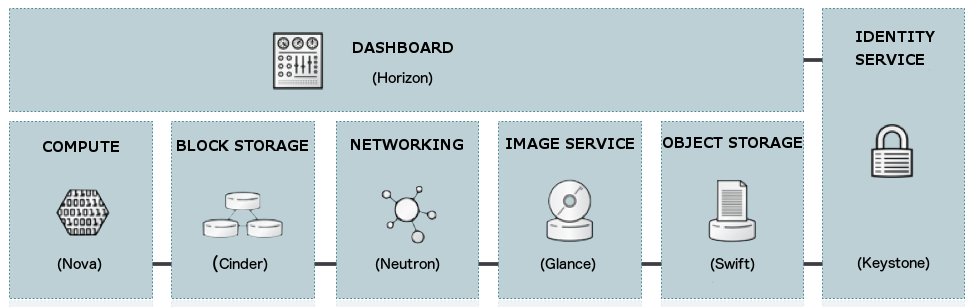
\includegraphics[width=\textwidth]{fig/openstack_services.png}
  \caption{OpenStack core services [Source: \cite{ServicesImageSource}]}
  \label{fig:openstack_services}
\end{figure}
OpenStack is composed of several components \cite{CL210} called services, which can be seen on picture \ref{fig:openstack_services}, and are also described in this section.
\begin{itemize}
  \item{\textbf{Horizon (dashboard)} is a web interface for managing OpenStack services providing graphical user interface. Horizon supports operations like launching instances, managing networking, and setting access controls.}
  \item{\textbf{Keystone (identity)} is a centralized identity service providing authentication and authorization for other services. It also provides a catalogue of services running in the OpenStack cloud.}
  \item{\textbf{Neutron (networking)} provides virtual networking infrastructure in the OpenStack cloud, including networks, subnets and routers. Other advanced services such as firewalls, virtual private networks (VPN) or quality of service (QoS) are also supported. This service handles the creating and management of the networking infrastructure for the cloud administrator and users.}
  \item{\textbf{Cinder (block storage)} manages persistent block storage volumes used by virtual machines. The service supports creating of snapshots which can be used for backing up data. Then backup can be then used to restore data or to create some new block storage volumes. This service is often used by the virtual machines as a storage.}
  \item{\textbf{Swift (object storage)} provides an object storage that allows users to store and retrieve files. Swift has a distributed architecture that enable horizontal scaling and redundancy. Data replication is managed by software, which allows larger scalability and redundancy than dedicated hardware.}
  \item{\textbf{Glance (image)} is a registry of virtual machine images. Users can copy server images and use them as templates when setting up new virtual servers.}
  \item{\textbf{Nova (compute)} is a service that manages virtual machines running on compute nodes. Nova is designed to scale horizontally on standard hardware and to download images to launch new instances. Nova is a distributed component that interact with Keystone for authentication, Glance for images and Horizon for a web interface. It uses libvirtd, qemu, and kvm for the hypervisor.}
  \item{\textbf{Ceilometer (metering)} is a service that provides a centralized source for metering and monitoring data, which can be used to meter and bill users.}
  \item{\textbf{Heat (orchestration)} an advanced service to orchestrate multiple cloud application using the Amazon Web Services (AWS) template format. The software integrates other core components of OpenStack into a one-file template system. Templates can be used to create most of OpenStack resources, such as instances, floating IPs, volumes, security groups or users. Heat also offers advanced functionality such as high availability, auto scaling and nested stacks.}
\end{itemize}

\section{Ansible}

\subsection{What is Ansible}
Ansible is an IT automation engine which can be used as a configuration management tool, for application deployment, orchestration of deployment and provisioning new servers, all of which will be described later in the section. \cite{AnsibleOverview}

\subsubsection*{Configuration management}
Configuration management typically means writing some kind of description of our servers - a state in which we want the servers to be. This definition of a state can include information about packages that should be installed (or, more precisely, present) on the server, configuration files containing specific values and have specific permission and ownership, that the correct services are running, and so on.

Except Ansible, common configuration management tools are for example Chef, Salt, or Puppet.  \cite{UpAndRunning}

\subsubsection*{Deployment}
Application deployment is a process of taking a source code of a software that has been written internally, building it to get the binaries, copying the required files to the servers that are supposed to run the application, and then starting the necessary services.

Tools other than Ansible that can be used for deployment are for example Capistrano, or Fabric, which are both open-source. \cite{UpAndRunning}

As Ansible can manage both deployment and configuration management, using a same tool for these tasks can make it easier and well-arranged for the people using it.

\subsubsection*{Orchestration of deployment}
We need to use orchestration when there are more servers involved and we need to run tasks in a specific order. This can mean, for example, bringing up the database server first and then starting the web servers. Or in case of updating web servers, we need to take them out of the load balancer one at a time to preserve stable service without outages.

Ansible is designed to support orchestration by using a simple model of dependencies build directly into the core architecture - so the tasks are automatically executed in the correct order.

\subsubsection*{Provisioning}
The term provisioning a new server is often used in a cloud environment. It means creating a new virtual machine instance with operating system installed and having the networking and access configured in a way that the machine can be used.

However, provisioning is also used with baremetal machines, because, in the end, all virtual and cloud machines run on a physical server. Ansible can provision all the machines in the datacenter and can be also integrated with several dataentre management tools, like (not limited to) Red Hat Satellite, Hanlon, or Cobler.

Ansible supports several cloud providers including Amazon EC2, Microsoft Azure, Digital Ocean, Google Compute Engine, Linode, Rackspace and clouds supporting the OpenStack APIs. \cite{UpAndRunning}

\subsection{Advantages of the Ansible Technology}
There are several features of the Ansible technology that are important to mention:

\subsubsection{Syntax is Easy to Read}
The ansible configuration management scripts are called playbooks. Playbooks and their structure will be described later in this section. Important to know right now is that they are build on top of YAML syntax, which is a data format language that was designed to be easy to read for people.

When used properly, the ansible playbooks might be seen as an executable documentation. And it will never be outdated, because it is also the code, that gets executed.

\subsubsection*{No Agents Required}
To manage a server by ansible, it only needs a Python version 2.5 or later and an SSH to be installed. Ansible does not need any agents or additional software to be installed on the servers. It also does not need any special management interfaces, as it runs on the existing network infrastructure using SSH.

\subsubsection*{Push-based mechanism}
There are two main concepts of deploying a change to servers: push-based and pull-based mechanisms.

Some configuration management, that use agents, are pull-based. An example of these tools can be Puppet or Chef. The pull-based mechanism work in the following way:
\begin{enumerate}
  \item{Administrator makes change to the configuration scripts}
  \item{Administrator pushes the changes to a central service}
  \item{Agent running on the server checks for changes periodically}
  \item{Agent downloads the change from the central service}
  \item{Agent executes the configuration script locally and changes the state of the server}
\end{enumerate}
Ansible uses the push-based mechanism, in which the administrator controls when a change is applied to the server. \cite{UpAndRunning} The administrator does not need to wait for a timer to expire before the change is applied. This is an advantage of the Ansible solution, as it offers more control over the overall system. The push-based mechanism works in the following way:
\begin{enumerate}
  \item{Administrator makes change to the configuration scripts}
  \item{Administrator runs the playbook}
  \item{Ansible connects to the servers and executes modules, making changes to the server}
\end{enumerate}
Ansible, however, also supports a pull-based mechanism, using a tool called ansible-pull.

\subsubsection*{Thin Layer of Abstraction}
Some configuration management tools provide a thick layer of abstraction, which enables the administrator to manage multiple operation systems using a single script. For example, an abstraction called package could be used to install a package on a system, regardless its type. It could be a yum-based, or a apt-based system. However, these abstractions can be even bigger.

Ansible does not use these kind of abstractions. This allows the administrator to write scripts for a specific system without the need of learning the abstractions, which makes the learning process shorter, and reading the scripts easier. \cite{UpAndRunning}




\subsection{Ansible Playbooks}
As already mentioned previously, ansible configuration scripts are called playbooks. Playbooks can define the configuration of the target servers, and they can orchestrate the steps in which the configuration is applied. Playbooks consist of several parts: plays, tasks, and modules. \cite{UpAndRunning} \cite{AnsibleDoc}

\begin{figure}[!h]
  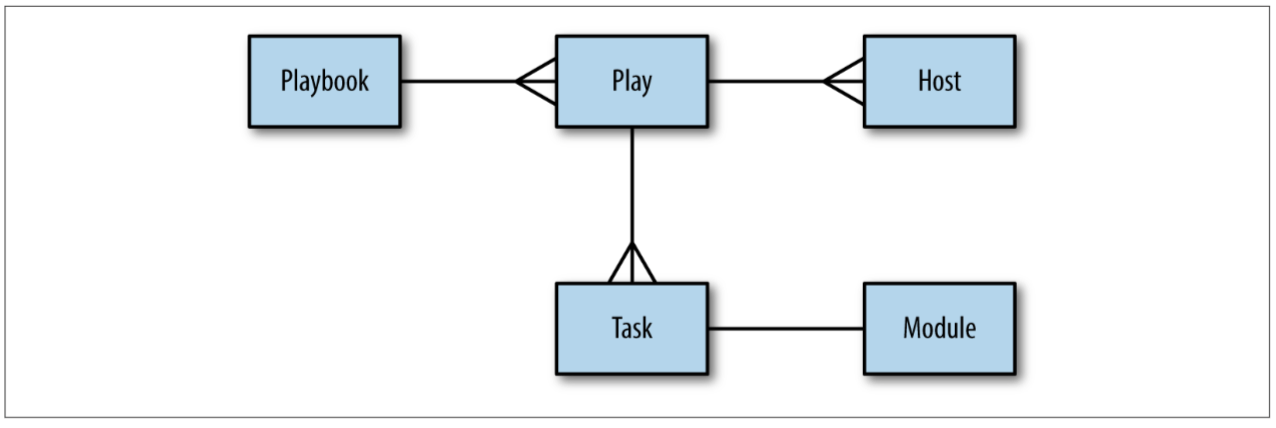
\includegraphics[width=\textwidth]{fig/playbook_anatomy.png}
  \caption{Ansible playbook anatomy [Source: \cite{UpAndRunning}]}
  \label{fig:playbook_anatomy}
\end{figure}

\subsubsection*{Plays}

Playbook is a list of plays. Plays can be thought of as a connection of tasks to hosts. A play must contain:
\begin{itemize}
  \item{A list of hosts}
  \item{A list of tasks that would be executed on the hosts}
\end{itemize}
Plays also support several optional settings that affect the way it is executed. An example of these settings can be:
\begin{itemize}
  \item{\texttt{name} - A description of the respective task. The names should be always used, as they will be printed} at the time of run, showing what changes has been made to a particular server.
  \item{\texttt{sudo} - A boolean value determining if the tasks will be executed with root privileges.}
  \item{\texttt{vars} - A list of variables that would be used for the particular task. They act as a parameters.}
\end{itemize}
An example of a play is shown below:

\begin{lstlisting}
- name: Configure webserver with nginx
  hosts: webservers
  sudo: True
  tasks:
    - name: install nginx
      apt: name=nginx update_cache=yes

    - name: copy nginx config file
      copy: >
        src=files/nginx.conf
        dest=/etc/nginx/sites-available/default

    - name: enable configuration
      file: >
        dest=/etc/nginx/sites-enabled/default
        src=/etc/nginx/sites-available/default
        state=link

    - name: copy index.html
      template: >
        src=templates/index.html.j2
        dest=/usr/share/nginx/html/index.html mode=0644

    - name: restart nginx
      service: name=nginx state=restarted
\end{lstlisting}
\cite{UpAndRunning}


\subsubsection*{Tasks}

Play is a list of tasks. Every task represents a single module that would be executed. Every task must contain:
\begin{itemize}
  \item{A name of the particular module}
  \item{A list of arguments for the module}
\end{itemize}

Task can also include a definition of its name. Using of names is a good practise, as they are printed at the time of run and can be used to track changes made by the scripts. They also act as comments, improving readability of the playbook.

\subsubsection*{Module}

Modules are scripts that perform the desired action on the target server.

They are designed to be idempotent, which means that they can be run multiple times, but will only make changes when there is a difference between the present and desired state. In other words, running a playbook for the second time without making changes will not affect the target server in any way.

An example of modules can be:
\begin{itemize}
  \item{\texttt{copy} - Copies a file from the local machine to the remote host.}
  \item{\texttt{service} - Manages the services running on the remote host. It can start, stop, or restart a services.}
\end{itemize}



\subsection{Tracking of Host State}

When ansible execute modules on a particular server, they may or may not make a change. They only make change when the present state is different from the desired state. At the time of run, ansible prints out the names of tasks that are being executed. If the state has changed, the module will return changed state. And if no action was needed, an ok state will be returned instead. Ansible will then print the result, as seen on the following example:

\begin{lstlisting}
TASK: [Install packages] **********************************
changed: [webserver1]

TASK: [Set configuration] *********************************
ok: [webserver1]
\end{lstlisting}

\subsubsection*{Handlers}

This detection of a change can be used by a mechanism called handlers. \cite{UpAndRunning} Handlers are actions triggered at the end of run only when a specific change has occurred. However, the action will be executed only once.

For example, a change of a web server configuration might require restart of the respective service. Also, an update of the web server package might require a restart of the service. If any of these actions occur, a handler responsible for restarting the service will be notified and executed at the end of run. It will be executed only once, even when both of the changes above will occur.

\subsection{Roles}

When managing a large number of servers, a single playbook describing changes of all of the servers would become too long and hard to maintain. Also, applying a common configuration to multiple servers would result in a duplication of code. To solve this problem, a mechanism called Roles has been introduced to Ansible. \cite{AnsibleDoc}

Roles are the main mechanism to break large playbooks into multiple files, which simplifies writing complex playbooks. It also makes them easier to reuse.

A role can be thought of as something that should be assigned to one or more hosts. For example, a database role will be assigned to servers acting as a database servers.

Roles can also be dependent, which means that a role can require other role to be applied before. Using this feature, Ansible will automatically ensure that roles are applied in the correct order.
